\documentclass[11pt]{exam}

\usepackage{amsmath}
\usepackage{graphicx}
\usepackage{geometry}
\usepackage{etoolbox}
\BeforeBeginEnvironment{choices}{\par\nopagebreak\minipage{\linewidth}}
\AfterEndEnvironment{choices}{\endminipage}
\geometry{
a4paper,
total={185mm,257mm},
left=10mm,
top=25mm,
bottom=10mm
}

\begin{document}
\setlength{\voffset}{-0.5in}
\setlength{\headsep}{5pt}

\fbox{\fbox{\parbox{8cm}{\centering
\vspace{2mm}
Testat - Versuch J - Ultraschall - 1
\vspace{2mm}
}}}
\hspace{2mm}
\makebox[0.25\textwidth]{Name:\enspace\hrulefill} \hspace{5mm}
\makebox[0.2\textwidth]{Datum:\enspace\hrulefill}
\vspace{4mm}

\begin{questions}

\question Wie groß ist die Wellenlänge des in der Graphik dargestellten Schallsignals (in Luft)? 

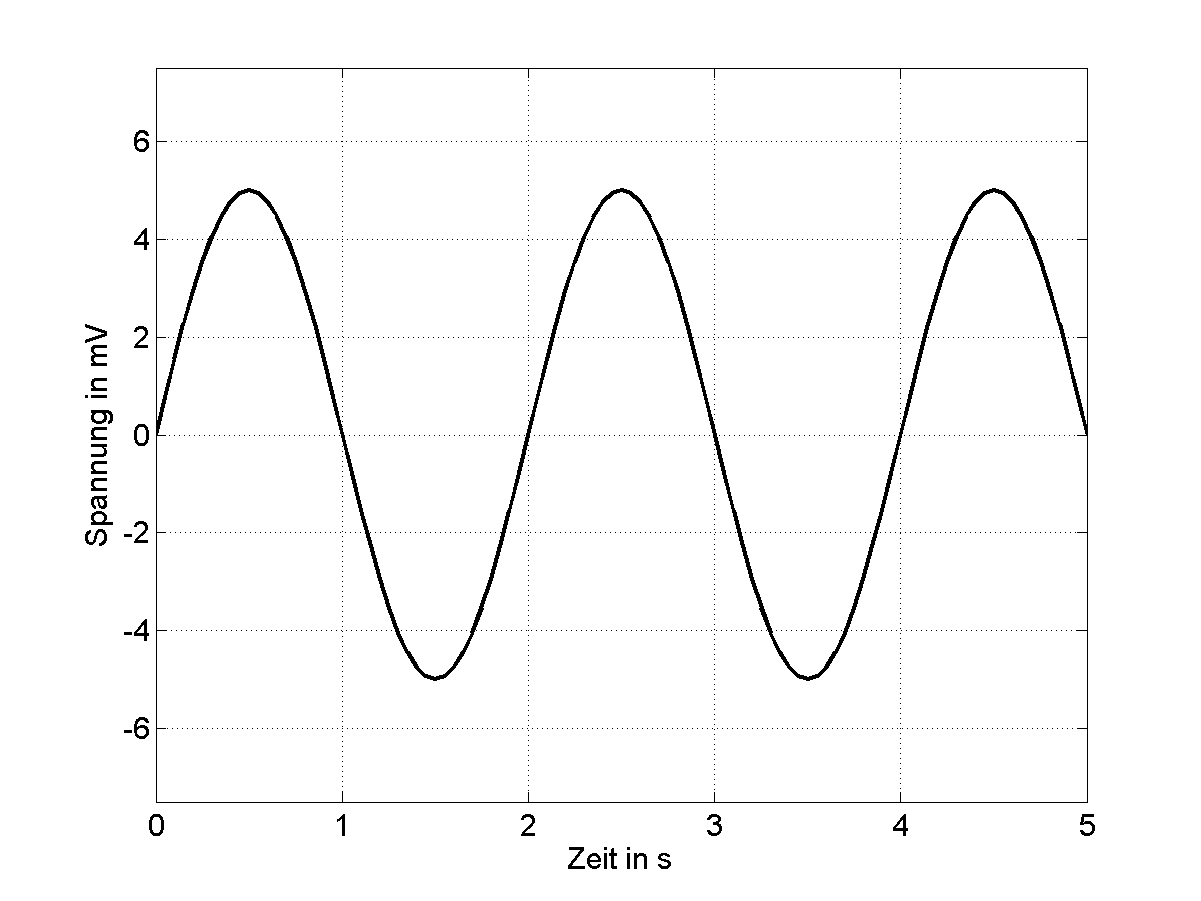
\includegraphics[width=0.5\textwidth]{../../../questions/J/images/SchallSinus2.png}

\begin{choices}
	\choice 34,3 m
	\choice 2 s
	\choice 686 m
	\choice 0,5 Hz
	\choice 343 m
\end{choices}

\vspace{3mm}\question Welcher Zusammenhang besteht zwischen Frequenz \( f \) und der Periodendauer \( T \) ?

\begin{choices}
	\choice Die Frequenz ist proportional zur Periodendauer.
	\choice Die Frequenz ist das Quadrat der Periodendauer.
	\choice Die Frequenz ist die Quadratwurzel aus der Periodendauer.
	\choice Die Frequenz ist das Doppelte der Periodendauer.
	\choice Die Frequenz ist das Inverse der Periodendauer.
\end{choices}

\vspace{3mm}\question Mit einem Echolot soll eine Position eines Gegenstandes in einem Medium mit einer Schallgeschwindigkeit von 100 m/s überprüft werden. Dazu wird durch eine Sonde eine Schallwelle ausgestrahlt, die an dem Gegenstand reflektiert wird und daraufhin wieder an der Sonde eintrifft. Wie lange müsste es bei einer Entfernung zwischen Gegenstand und Sonde von 25~m dauern, bis die Schallwelle nach ihrer Aussendung wieder an der Sonde eintrifft?

\begin{choices}
	\choice etwa 0,25 s
	\choice etwa 1 s
	\choice etwa 0,5 s
	\choice etwa 4 s
	\choice etwa 2 s
\end{choices}

\vspace{3mm}\question Der piezoelektrische Effekt...

\begin{choices}
	\choice bewirkt, dass sich ein Körper beim Anlegen einer elektrischen Spannung sehr stark erwärmt.
	\choice bewirkt, dass sich ein Körper beim Anlegen einer elektrischen Spannung mechanisch verformt.
	\choice ist nicht umkehrbar.
	\choice bewirkt, dass Schallwellen an ebenen Flächen reflektiert werden.
	\choice ist bei Raumtemperatur vernachlässigbar.
\end{choices}

\vspace{3mm}\question Welche Aussagen zur Ultraschalldiagnostik sind zutreffend?	* Ultraschallgeräte funktionieren nach dem Prinzip der Laufzeitbestimmung  von Ultraschallpulsen.	* Trifft ein Ultraschallpuls auf eine Grenzfläche zwischen zwei Medien, so wird der Schall daran immer vollständig reflektiert. So entsteht ein Echo, das für die Laufzeitbestimmung genutzt werden kann.	* In einem Ultraschallgerät sind meistens zwei verschiedene Geräte, ein Ultraschall-Sender und ein Ultraschall-Empfänger, eingebaut.	* Die Reflexion von Ultraschallwellen an Gewebegrenzflächen kann mit dem aus der Optik bekannten Reflexionsgesetz beschrieben werden.

\begin{choices}
	\choice Nur 2 und 3 sind richtig.
	\choice Nur 1 und 2 sind richtig.
	\choice Nur 1 und 4 sind richtig.
	\choice Nur 4 ist falsch.
	\choice Nur 2 ist falsch.
\end{choices}

\vspace{3mm}\end{questions}

\end{document}
